\section{Real-time performance}
\label{sec:prediction_performance}

The primary constraint on real-time applications is time, especially when the predictions will be out of date once the next vehicle observations are available 30~seconds after the first. We recorded the timings of each component of our application during the simulation described in \cref{sec:prediction_model_comparison}. \Cref{tab:prediction_timing} presents the mean timing results for each component using both \emph{wall clock} (the time passed as recorded by a clock on the wall), as well as the \emph{CPU clock} (the processing time). The latter represents the overall computational complexity of the problem. Since computations are spread out over multiple cores (in this simulation we used 3)  the actual wall clock is up to 33\% faster in the vehicle update, network update, and \gls{eta} prediction steps (we discussed multithreading in \cref{sec:rt-implementation}). In some steps (such as while loading data), the wall clock time is longer than the CPU time: this is because the step involved downloading data from the server, during which time the processor is mostly inactive while it waits for the file.



\begin{knitrout}\small
\definecolor{shadecolor}{rgb}{0.969, 0.969, 0.969}\color{fgcolor}\begin{table}

\caption{\label{tab:prediction_timing}Time taken, in milliseconds, during various parts of the program, running on a single core.}
\centering
\fontsize{8}{10}\selectfont
\begin{tabular}[t]{lrlrl}
\toprule
 & Wall clock & (SE) & CPU time & (SE)\\
\midrule
(L) Load data & 28.1 & (0.22) & 16.7 & (0.19)\\
(U) Update vehicle information & 3.47 & (0.04) & 3.32 & (0.034)\\
(V) Vehicle state update & 3930 & (37) & 10400 & (96)\\
(N) Network state update & 0.874 & (0.12) & 1.6 & (0.026)\\
(P) Predict ETAs & 1650 & (26) & 3490 & (39)\\
\addlinespace
(W) Write ETAs to protobuf feed & 327 & (1.5) & 341 & (1.1)\\
\midrule
(T) Total iteration time & 5940 & (55) & 14200 & (130)\\
\bottomrule
\end{tabular}
\end{table}


\end{knitrout}


From the results in \cref{tab:prediction_timing}, we see that the average iteration time is about 6~seconds, which is well below our original target of 30~seconds. The CPU time is about 14~seconds, so, on average, we see a 50\% reduction attributed to multithreading on three cores. The most computationally intensive step is the vehicle state update, which involves transitioning, reweighting, and occasionally resampling 5000~particles for each vehicle, which can exceed 1000 at peak time. Next is the arrival time prediction step, which also involves estimation with a subset of particles (in this simulation, we used 200). The last significant step is writing the \glspl{eta} to file, which additionally (in this case) involved computing the median arrival time for each vehicle and stop combination (\cref{app:particle-summaries}). The remaining steps each had average times of less than 0.1~seconds.



\begin{knitrout}\small
\definecolor{shadecolor}{rgb}{0.969, 0.969, 0.969}\color{fgcolor}\begin{figure}

{\centering 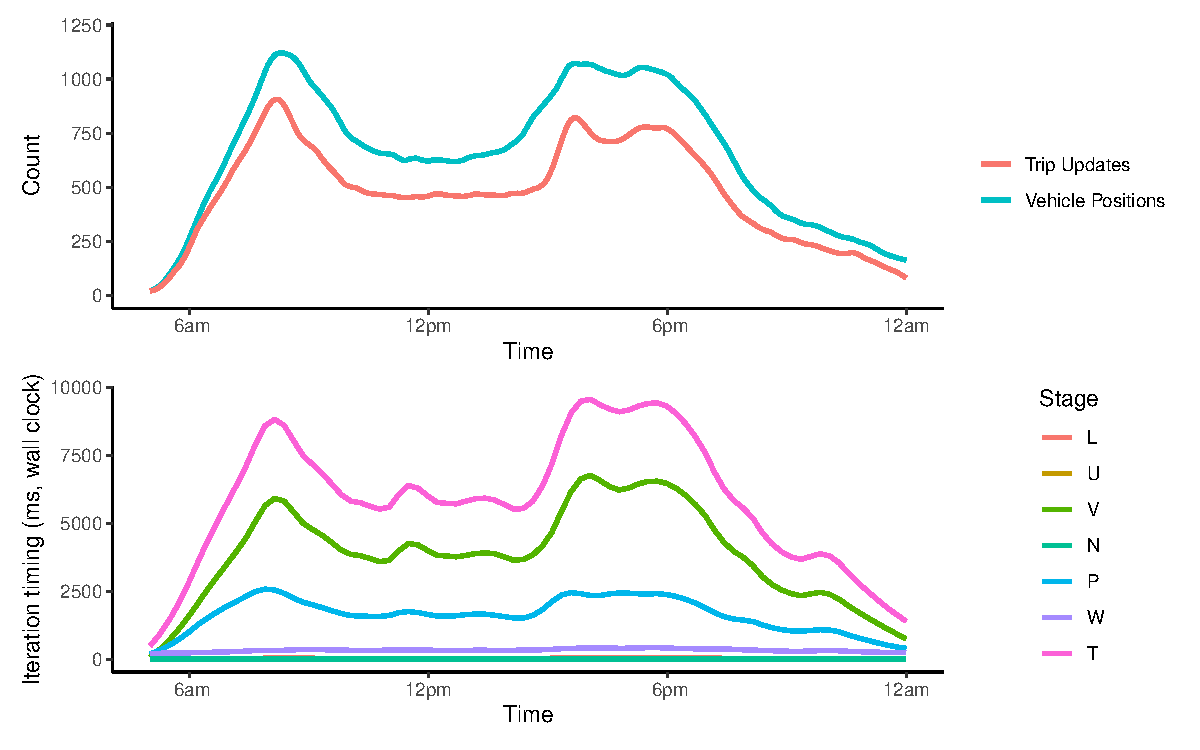
\includegraphics[width=\textwidth]{figure/prediction_timing_time-1} 

}

\caption[Number of vehicles and trip updates at different times ofthe day, along with the timing results over time for various stages of the program]{Number of vehicles and trip updates at different times ofthe day, along with the timing results over time for various stages of the program: (L) Load data, (O) Update vehicles information, (V) Vehicle state update, (N) Network state update, (P) Predict ETAs, (W) Write ETAs to protobuf feed, (T) Total iteration time.}\label{fig:prediction_timing_time}
\end{figure}


\end{knitrout}



Since the number of vehicles changes throughout the day, as displayed in the top half of \cref{fig:prediction_timing_time}, we also display the timings over time, as shown in the lower half of the figure. We see the two peak periods: morning peak, which includes both school and workers at the same time, and the broader evening peak since schools finish at about 3~pm while most workers finish about 5~pm. When the number of vehicles exceeds 1100, the total iteration time is around 9~seconds and remains at around 6~seconds during daytime off-peak. Again, this is the wall clock iteration time, so deployment on a server with more cores would result in even faster iterations.
